\documentclass[12pt]{article}

\usepackage[french]{babel} % Document en français
\usepackage[T1]{fontenc} % Suppression d'un warning
\usepackage[utf8]{inputenc} % Document UTF8
\usepackage{graphicx} % Insertion d'images
\usepackage[left=2.2cm, right=2.2cm, top=2.5cm, bottom=2.5cm]{geometry} % Mise en page
\usepackage{multicol} % Texte en multicolonnes avec multicols
\usepackage{placeins}

\graphicspath{{res/}}

\title{LECGE1321 - Management Humain}
\author{Florian Thuin}


\begin{document}

\maketitle
\tableofcontents

\section{Introduction}

\section{Panorama historique et rôles de la fonction RH}
	\subsection{Les étapes historiques}
		\subsubsection{L'administration du personnel}
		\subsubsection{L'approche socio-technique}
		\subsubsection{La gestion des ressources humaines}

\section{Culture organisationnelle}
	\subsection{Historique}
	\subsection{Le modèle de l'oignon d'Edgar Schein}
	
	Le modèle d'Edgar Schein est une conceptualisation de la notion de culture d'entreprise via une approche anthropologique.
	
	Pour Edgar Schein, la culture organisationnelle se définit comme \og{} un ensemble de prémisses et de croyances partagées que le groupe a appris au fur et à mesure qu'il a résolu ses problèmes d'adaptation externe et d'intégration interne, qui a fonctionné suffisamment bien pour qu'il soit considéré valide, et par conséquent est enseigné aux nouveaux membres comme la manière appropriée de percevoir, de penser et de ressentir par rapport à ces problèmes \fg{} \cite{schein2010}
	
	  \subsubsection{Un phénomène multi-niveaux}
	  
	  Edgar Schein divise la culture d'une entreprise en plusieurs niveaux :
	  
	  \begin{multicols}{2}
	  
	  Les \textbf{artéfacts} sont les aspects visibles de la culture : la manière de s'habiller, les logos, le jargon, l'humour,... Ils sont faciles à identifier par une démarche ethnographique mais il est difficile d'en tirer une signification sans analyser les autres niveaux de l'oignon.
	  
	  Les \textbf{valeurs} sont les stratégies, les objectifs et philosophies choisies de manière consciente et qui sont diffusées par la direction et le management de l'entreprise : compétitivité, solidarité, adaptation au changement, stabilité, etc.
	  
	  Les \textbf{normes de pensée et d'action} correspondent aux routines comportementales, habitudes, modèles d'action, rituels et schémas cognitifs d'inteprétation des évènements. Elles sont directement déterminées par les valeurs sous-jacentes.
	  	  
	  \begin{center}
	    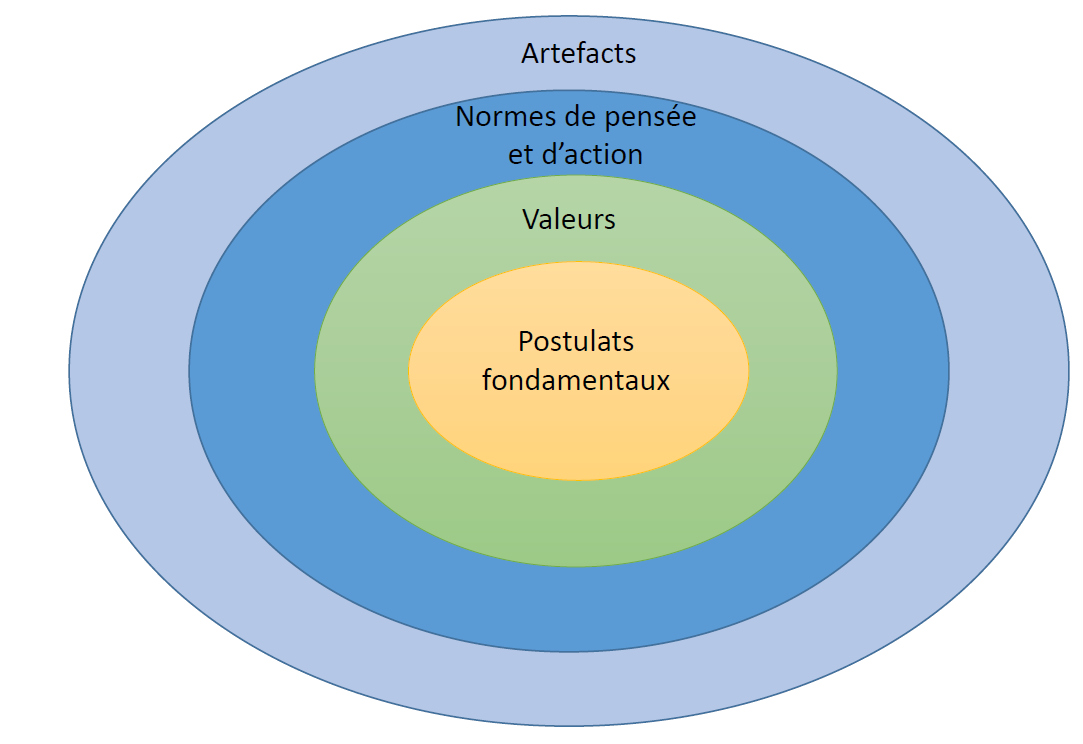
\includegraphics[width=\linewidth]{culture_orga_niveaux.png}
	  \end{center}
	  Les \textbf{postulats fondamentaux} ou prémisses sont les croyances qui sont l'essence de la culture. Ces prémisses sont difficiles à discerner car elles opèrent au niveau de l'inconscient. Elles portent sur des questions telles que la nature de l'homme, le rapport au temps, la notion de vérité, etc. Elles ne sont quasiment jamais remises en cause.
	  
	  Les artéfacts découlent des valeurs et les valeurs découlent des postulats fondamentaux.
	  
	  \end{multicols}
	  
      \subsection{Le modèle des valeurs concurrentes de Quinn}
	Ce modèle a été développé à l'origine pour décrire les valeurs sous-jacentes aux critères d'efficacité organisationnelle.
	
	Il caractérise les cultures organisationnelles selon 2 dimensions : le contrôle VS la flexibilité et les relations (interne) VS les résultats (externe).
	
	\subsubsection{Un phénomène multi-dimensionnel}
	
	  Quinn définit 4 grands types de cultures :
	  
	  La \textbf{culture de soutien} qui privilégie la coopération, la participation, l'attachement à l'entreprise, la communication interpersonnelle. C'est une culture de \og{} collaborateurs \fg{} qui peut se retrouver notamment dans les PME familiales.
	  
	  La \textbf{culture des règles} qui est très respectueuse des procédures, tout est écrit, tracé, standardisé. La communication est essentiellement descendante dans l'organigramme, c'est une culture \og{} d'organisateurs \fg{}. Cette culture peut se retrouver dans les administrations publiques.
	  
	  La \textbf{culture des buts} privilégie les objectifs de performance et la rationalisation des processus en vue des objectifs. C'est une culture de \og{} compétiteurs \fg{}. 
	  
	  La \textbf{culture de l'innovation} qui privilégie la créativité, l'ouverture au changement, l'expérimentation et l'adaptation permanente. La communication est aussi peu formalisée que possible pour casser la hiérarchie stricte, c'est une culture \og{} d'innovateurs \fg{}.
	  
	  Ce modèle peut se superposer à celui d'Ulrich pour tracer un historique des pratiques de ressources humaines.
	
	\subsection{La théorie des dimensions culturelles (1991)}
	
	Une organisation (de taille conséquente) n'est pas liée à une seule culture, il existe des sous-cultures. Il y a les sous-cultures par département, par métiers, par âge, par affinités,...
	
	  \subsubsection{Un phénomène hétérogène}
	  
	  Le modèle de Hofstede a pour but d'étudier les interactions entre les cultures en fonction de certaines dimensions en leur attribuant des scores de 1 à 120.
	  
	  Il met en avant 4 dimensions :
	  
	  \begin{enumerate}
	   \item Distance au pouvoir
	   \item Evitement de l'incertitude
	   \item Masculinité contre féminité
	   \item Individualisme contre collectivisme
	  \end{enumerate}
	  
	  La \textbf{distance au pouvoir} est un indice d'acceptation de pas avoir de pouvoir par les membres les plus éloignés de la direction dans l'organigramme.
	  Un indice faible signifie que les membres souhaitent une gestion démocratique et se considèrent à égalité avec les autres, un indice élevé indique que ceux qui ont le moins de pouvoir acceptent leur condition et sont forts soumis au pouvoir.
	  
	  L'\textbf{évitement de l'incertitude} correspond au degré de tolérance d'une société pour l'incertitude/l'ambiguité. Les sociétés avec un indice faible sont ouvertes aux changements, disposent de moins de règles et de lois et les directives y sont plus souples.
	  
	  La \textbf{masculinité contre la féminité} correspond au niveau d'importance accordée aux valeurs masculines (assurance, ambition, pouvoir, matérialisme) et aux valeurs féminines (égalité, relations humaines).
	  
	  L'\textbf{individualisme contre le collectivisme} correspond au degré auquel les individus sont intégrés aux groupes. Une culture individualiste donne de l'importance à l'initiative privée et la réussite d'objectif personnels, une culture collectiviste met en avant le bien-être du groupe, la loyauté, l'intérêt collectif avant l'intérêt personnel.
	  
	  Il est possible de croiser les dimensions entre elles.
	  
	  L'analyse pour la culture belge pourrait donner ceci : une distance au pouvoir plutôt forte, un évitement de l'incertitude fort, une légère prédominance masculine et une culture plutôt individualiste.
	  
	  \begin{figure}[!ht]
	   \begin{center}
	    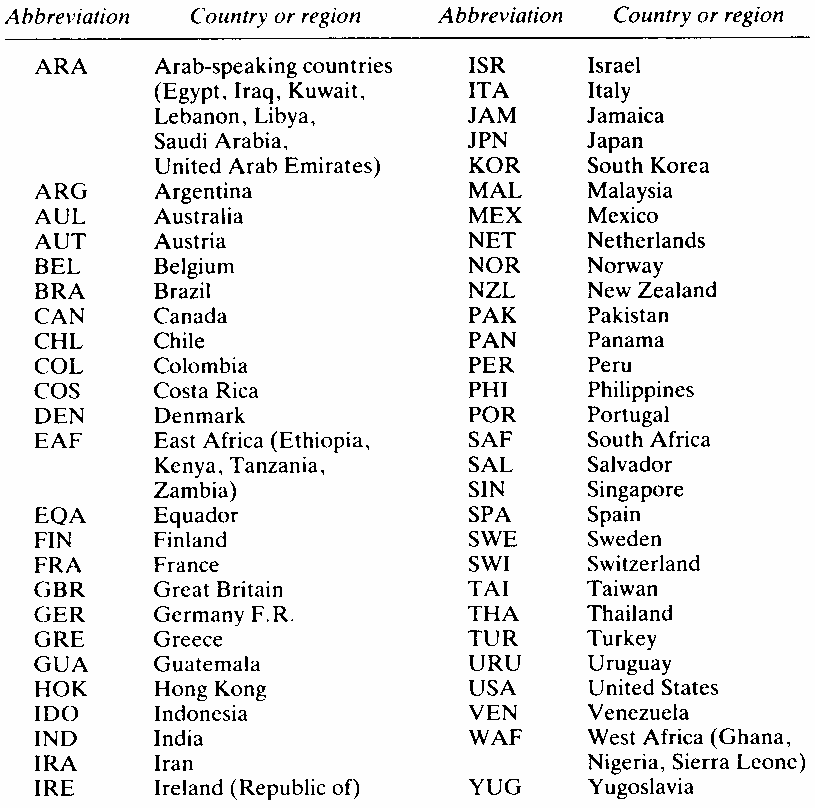
\includegraphics[width=0.65\linewidth]{hofstede_abbr.png}
	    \caption{Abréviations pour les pays et régions étudiés}
	   \end{center}
	  \end{figure}
	  
	  \begin{figure}[!ht]
	   \begin{center}
	    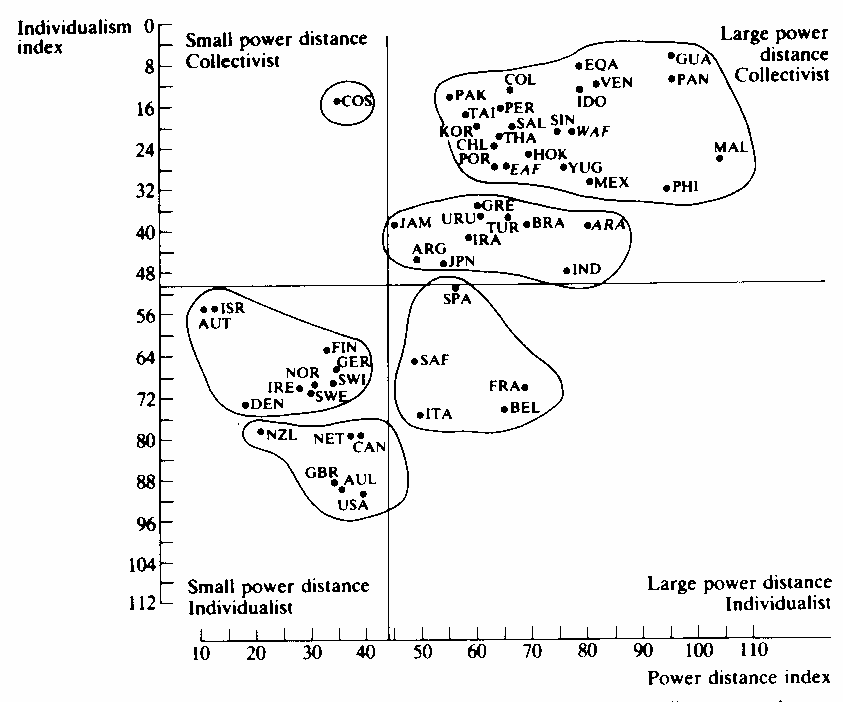
\includegraphics[width=0.65\linewidth]{hofstede_indivi_collect.png}
	    \caption{Position des 50 pays et 3 régions sur la distance au pouvoir et l'individualisme-collectivisme}
	   \end{center}
	  \end{figure}
	  
	  \begin{figure}[!ht]
	   \begin{center}
	     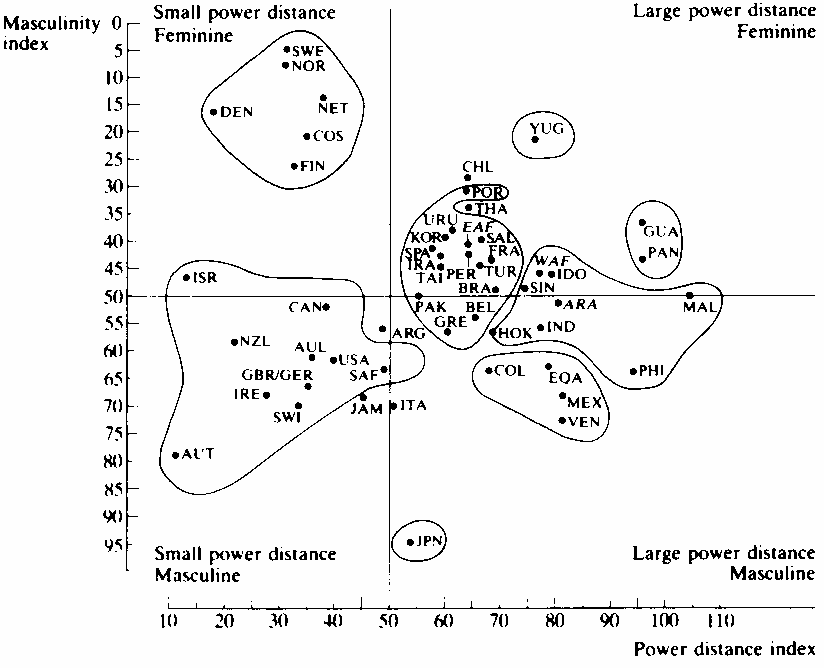
\includegraphics[width=0.65\linewidth]{hofstede_power_masc.png}
	     \caption{Distance au pouvoir contre masculinité pour 50 pays et 3 régions}
	   \end{center}
	  \end{figure}

	  \begin{figure}[!ht]
	   \begin{center}
	     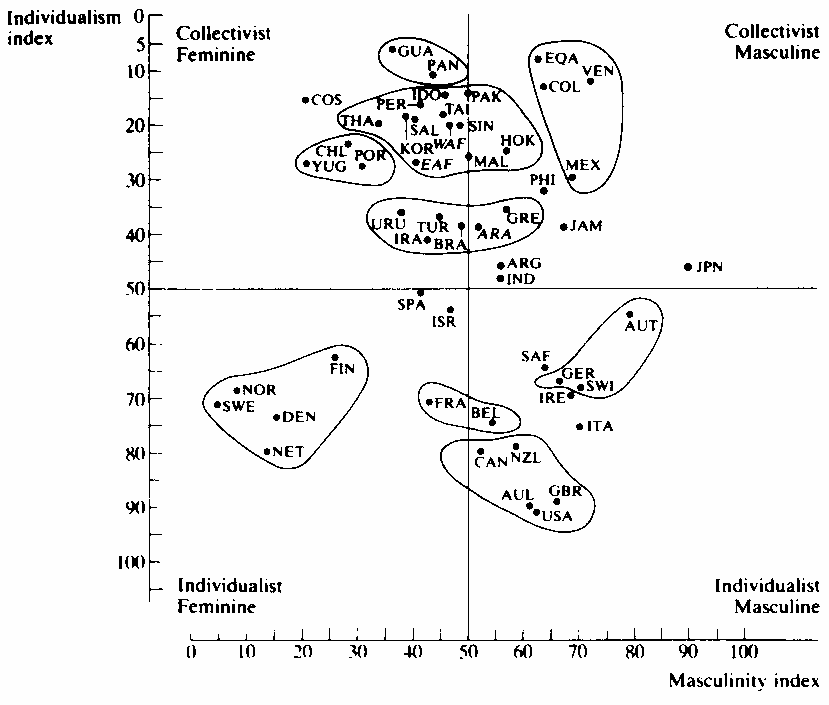
\includegraphics[width=0.65\linewidth]{hofstede_masc_indivi.png}
	     \caption{Position de 50 pays et 3 régions sur les dimensions masculinité-féminité et individualisme-collectivisme}
	   \end{center}
	  \end{figure}
	  
	  \begin{figure}[!ht]
	   \begin{center}
	    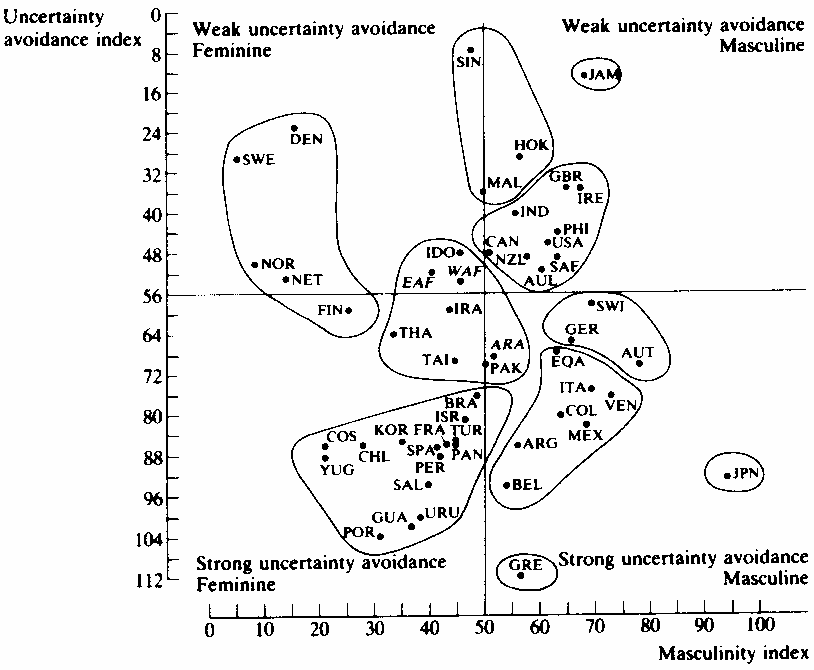
\includegraphics[width=0.65\linewidth]{hofstede_masc_incertitudes.png}
	    \caption{Position de 50 pays et 3 régions sur les dimensions masculinité/féminité et évitement de l'incertitude}
	   \end{center}
	  \end{figure}
	  
	  \begin{figure}[!ht]
	   \begin{center}
	    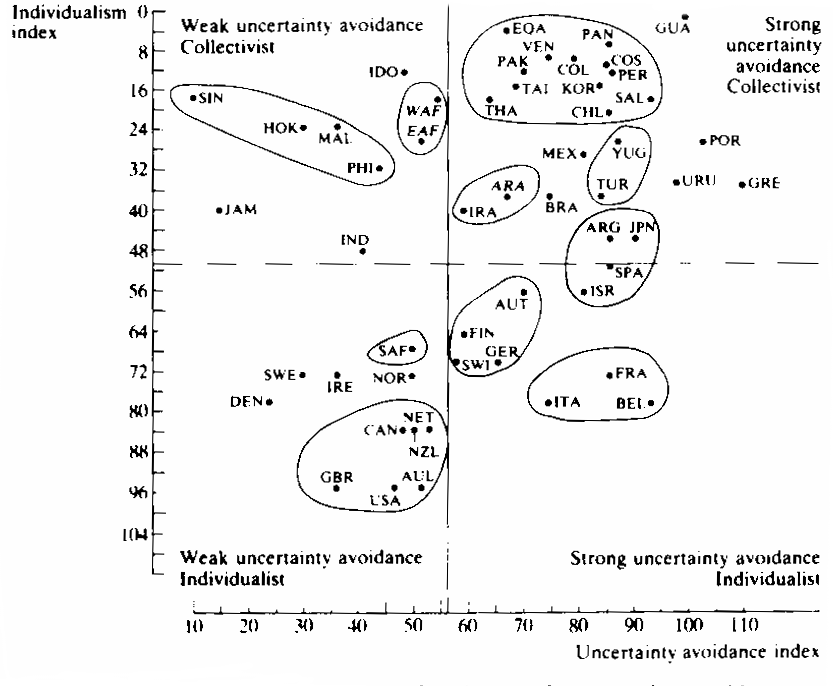
\includegraphics[width=0.65\linewidth]{hofstede_incertitudes_indivi.png}
	    \caption{Position de 50 pays et 3 régions sur les dimensions d'évitement d'incertitude et individualisme-collectivisme}
	   \end{center}
	  \end{figure}

	  \FloatBarrier % Force les flottants à se placer ici


	\subsection{Un phénomène dynamique}
	\subsection{Méthodologies d'étude}
	\subsection{Les répercussions}

\section{Leadership}

\section{Dynamique de groupe}

\section{Motivation au travail}

\section{Conclusion}

\bibliographystyle{plain}
\bibliography{biblio}


\end{document}